\documentclass[12pt,fleqn]{article}\usepackage{../../common}
\begin{document}
Saklı Markov Modelleri (Hidden Markov Models -HMM-)

Zaman serilerini temsil etmek için Markov bazlı modeller sıkça
kullanılır. Genelde istatistiki analiz bağımsız özdeşçe dağılmış (iid)
örneklem noktaları olduğunu farz eder, fakat çoğu zaman serisinde veri
noktaları birbirinden bağımsız değildir, $t$ anındaki bir nokta $t-1$
anındaki nokta ile bağlantılıdır. 

Saklı {\em olmayan} Markov modellerini, yani Markov Zincirlerini [5]'de
görmüştük. Bir MZ sistemi her $t$ adımında bir konumda (state) olan bir
sistem, $X_1,..,X_T$ rasgele değişkenleri ile temsil edelim, e bu modelde
bir konumdan diğerine geçiş belli olasılıklar üzerinden temsil edilir. Hiç
değişme olmaması da aslında bir geçiştir, bu durumda konum kendisine doğru
bir geçiş yapar. Matematiksel olarak bir konumdan diğerine geçme olasılığı

$$ P(X_t = j | X_{t-1} = i)  $$

ile gösterilir. Önceki adımda $i$ konumundayız, geçiş sonrası $j$'e
geliyoruz, $t$ anındaki konuma geçiş için sadece $t-1$'deki konumu bilmek
yeterlidir. Resme bakalım,

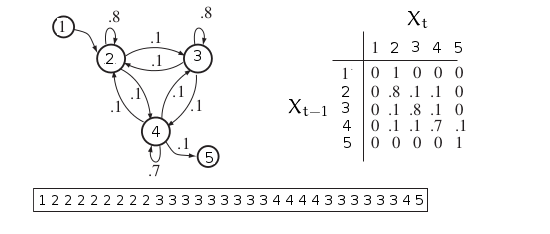
\includegraphics[height=5cm]{tser_hmm_01.png}

Konumlar ayrıksal, üstte 1,2,3 gibi değerler görülüyor. Bu değerler anlamı
olan yine ayrıksal bir alfabeyi indisliyor olabilirler. Mesela 1 belki
``araba'', 2 ``bisiklet'', 3 ``uçak'' gibi.  Geçiş olasılıkları bir $A$
matrisi içinde toplanabilir, resimde görüldüğü gibi, formülsel olarak

$$ P(X_t = j | X_{t-1} = i) = a_{ij} $$

Resimde ayrıca örnek bir konum serisi / dizisi de görüyoruz. Bu şekilde bir
seri bilinen MZ geçiş olasılıklarından ``üretilebilir''; bir başlangıç
konumu seçeriz, bir sonrakine geçiş olasılıklarına bakarız (5 tane), bu
olasılıklar üzerinden zar atarız, birini seçeriz, ve o konuma
geçeriz. İşlemi tekrarlarız. Böylece $X_1,X_2,..$ ``zincirini'' elde
ederiz.

Tam tersi yönde bir hesap yapmamız da gerekebilir; elde bir seri var, ama
$A$ bilinmiyor, o zaman konum dizisinden $A$ matrisini
``öğrenebiliriz''. Öğrenim için bildiğimiz maksimum olurluk hesabı
kullanılır, herhangi bir konum serisinin olasılığı nedir sorusunun cevabı
şu formül;

$$ P(X_1=x_1,..,X_T=x_T) = 
P(X_1=x_1) \prod _{t=2}^{T} P(X_t=x_t | X_{t-1}=x_{t-1})
$$

Üstteki formül bir olurluk (likelihood) hesabı - $L(A)$ diyelim, 

$$ L(A) = P(X_1=x_1) \prod _{ t=2}^{T} a_{x_{t-1},x_t} $$

Olurluğun maksimize edilmesi ardından $A$ için bir tahmin edici
(estimator) hesaplanabilir - detaylar için [2, Ders 6]; $n_{ij}$'yi veri
serisinde $i$'inci konumdan $j$'ye kaç kere geçildiğinin sayısı olarak
tanımlarsak, $A$ tahmin edicisi şöyle olur,

$$ \hat{a}_{ij} = \frac{n_{ij}}{\sum_j n_{ij}}  $$

Bu hesap akla yatkın (intuitive) bir sonuç, çünkü $i$'den $j$'ye geçiş
``olasılığını'' veriden hesaplamak istiyorsak, veride $i$'den $j$'ye kaç
kere geçildiğini sayıp, bu sayıyı yine verideki tüm $j$'ye olan geçişlere
(hangi konumdan olursa olsun) bölmek bize iyi tahmin sağlar. Bir
Gaussian'ın $\mu$'sünü tahmin ederken tüm reel veri noktalarını toplayıp
bölmek aynı şekilde akla yatkın bir tahmin edicidir.

Şimdi MZ kavramına bir ek daha yapalım. Diyelim ki bir katman daha
ekleyeceğiz, öyle ki artık konum geçişlerini dışarıdan göremiyoruz, sadece
konumların {\em başka bir dağılıma göre} dışarıya ürettiği farklı bir
alfabeden değerleri görüyoruz.

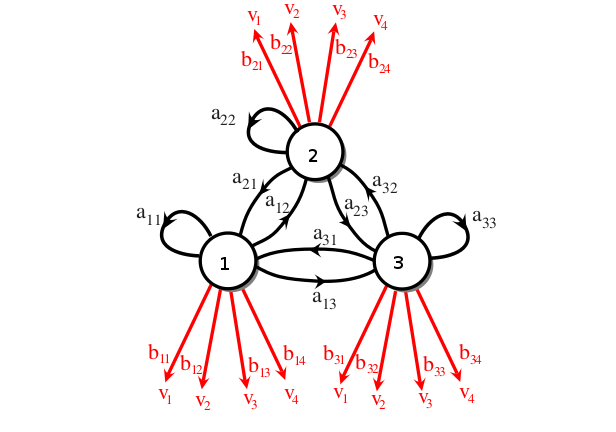
\includegraphics[height=8cm]{tser_hmm_02.png}

Konum geçişleri bu sayede ``saklı'' hale geldi, ve bir HMM elde
ettik. Matris olarak görelim,

$$ 
A = \left[\begin{array}{rrr}
a_{11} & a_{12} & a_{13} \\
a_{21} & a_{22} & a_{23} \\
a_{31} & a_{32} & a_{33} 
\end{array}\right], \qquad
B = 
\left[\begin{array}{rrrr}
b_{11} & b_{12} & b_{13} & b_{14} \\
b_{21} & b_{22} & b_{23} & b_{24} \\
b_{31} & b_{32} & b_{33} & b_{34} 
\end{array}\right]
$$

Üstteki model bir ayrıksal HMM örneğidir, yani hem saklı geçişler
ayrıksal (Markov durumunda hep öyle olmak zorunda) ve dışarı üretilen
değerler de ayrıksal. Dışarı yansıtılan / salımlanan (emission)
sembollerinden 4 tane var, $v_1,v_2,v_2,v_4$. Salımlar sürekli de
olabilirdi, mesela her konumun ayrı bir Gaussian dağılımı olabilirdi. Bu
konuya sonra değineceğiz. 

Not: Salım sembolleri olarak $v_1,v_2,..$ kullandık fakat matematik olarak
bunlar da aslında bir indis; saklı konumların aynı şekilde tamsayı olan
indisleri ile karışmaması için semboller seçildi. Tabii aynen saklı konumda
olduğu gibi salımların indisleri de herhangi bir alfabeyi
indeksleyebilir. Mesela 1 ``a'', 2 ``b'' olabilir. İndislerin direk kendisi
de kullanılabilir; mesela saklı konumlara bağlı zar atışlarını
modelliyorsak salımlar 1,2,3,4,5,6 olacaktır.

Devam edelim; HMM bu salım sembollerinden herhangi birini üretebilir, ama
her saklı konumda üretim farklı bir dağılıma göre olur. Bu dağılımları
içeren salım olasılıkları ayrı bir $B$ matrisi üzerinde tutulur. Matrisin
boyutu 3 saklı 4 görünen konum üzerinden $3 \times 4$ olmalıdır, ve
matrisin öğeleri $b_{jk}$'nin matematiksel tanımı,

$$ 
b_{jk} =  P (V_t = k | X_t = j )
$$

(Görüldüğü gibi üstte salım indisini kullandık). $V_t$ değişkeni $t$ anında
gizli $j$ konumunda olan bir HMM'in ürettiği semboldur. İki şarttan
bahsetmek lazım şimdi, bunlardan birincisi pür MZ durumunda da geçerli,

$$ \sum_j a_{ij} = 1, \quad \forall i$$

HMM ek bir şart,

$$ \sum_k b_{jk} = 1, \quad \forall j $$

Şimdi diyelim ki $V$ bir görünen sembol vektörü, $S_r$ ise $T$ boyutunda
bir saklı konum vektörü, ve bu boyutta olabilecek {\em tüm} konum
serilerini düşünelim, $c$ mümkün gizli konum için $c^T$ tane olur. $T=6$
için bir vektör $S_1 = \{1,4,2,2,1,4\}$ gibi.. Şimdi görünen herhangi bir
dizinin olasılığını hesaplayalım,

$$ P(V) = \sum _{r}^{c^n} P(V | S_r) P(S_r) 
\mlabel{1}
$$

Üstteki formüldeki $P(S_r)$'in açılımını MZ'lerden zaten biliyoruz, 

$$ P(S_r) = \prod _{t=1}^{T}P(X_t|X_{t-1}) $$

Yani gizli konum geçişlerine tekabül eden $a_{ij}$'leri bulup onları
sırasıyla çarpıyoruz. Üstteki $\{1,4,2,2,1,4\}$ örneği için bu
çarpım $a_{14}a_{42}a_{22}a_{21}a_{14}$ olurdu. 

Ayrıca $P(V|S_r)$'in açılımını da biliyoruz, 

$$ P(V|S_r) = \prod _{t=1}^{T} P(V_t | X_t) $$

Birleştirelim ve (1)'i genişletelim,

$$ 
P(V) = \sum _{r}^{c^T} \prod _{t=1}^{T} P(V_t | X_t)  P(X_t|X_{t-1}) 
$$

Formül biraz korkutucu duruyor ama aslında söylediği şu: verilen bir
$V$'nin olasılığını hesaplamak için tüm mümkün saklı konum dizileri
üzerinden bir toplam almalıyız, bu toplamdaki her dizi için $a_{ij}$
üzerinden gizli geçişlerin çarpımını alırız, sonra görünen salımların bir
çarpımını alırız, ki bu bilgi zaten $b_{jk}$ içinde. $A,B$ bilindiğine göre
tarif edilen işlemler direk yapılabilir.

Fakat bu hesap aşırı yüksek boyutlu bir hesaptır, çetrefilliği $O(c^T \cdot T)$, 
mesela $c=10,T=20$ olsa $10^{21}$ ölçeğinde bir hesaptan bahsediyoruz.
İçinde $c$ sembol olan bir alfabenin $n$ uzunluğunda çok fazla farklı dizilimi
mümkündür. 

İleri Algoritması (Forward Algorithm)

Fakat $P(V)$'yi literatürde ileri algoritması denilen bir yöntemle özyineli
(recursive) olarak hesaplamak mümkündür. Bakıyoruz her terim $P(V_t | X_t)
P(X_t|X_{t-1}) $için sadece $V_t,X_t,X_{t-1}$ gerekli. O zaman özyineli
hesap için  yeni bir  değişken tanımlarız, bilinen bir model 
$\lambda = (A,B)$ için

$$ \alpha_t(i) = P(V_1,V_2,..,V_t, X_t = i; \lambda) $$

Bu gözlenen salım dizisinin sadece bir kısmı üzerinden tanımlanmış bir
olasılık; tanıma göre zaman indisi 1'den $t$'ye kadar, ve bu en son $t$
noktasında saklı konum $i$'de olmalı. Özyineli tanımı görmek için
$\alpha_1(i)$'nin ne olduğuna bakalım, notasyon kısalığı için 
$\pi_i = P(X_1 = i)$,

$$ \alpha_1(i) = \pi_i b_{i,V_1} $$

Tümevarımsal (induction), özyineli kısım ise şöyle tanımlanır,

$$ \alpha_{t+1}(j) = \bigg[ \sum _{i=1}^{c} \alpha_t(i)a_{ij} \bigg] b_{j,V_{t+1}} $$

Formülün niye performans ilerlemesi getirdiğini görmek için örnek 1,2,3,4
gizli konumların tüm permutasyonlarının düşünelim,

\begin{minted}[fontsize=\footnotesize]{python}
import itertools
l = list(itertools.permutations([1, 2, 3, 4]))[:10]
for x in l: print x
print '...'
\end{minted}

\begin{verbatim}
(1, 2, 3, 4)
(1, 2, 4, 3)
(1, 3, 2, 4)
(1, 3, 4, 2)
(1, 4, 2, 3)
(1, 4, 3, 2)
(2, 1, 3, 4)
(2, 1, 4, 3)
(2, 3, 1, 4)
(2, 3, 4, 1)
...
\end{verbatim}

Mesela $t=2$'de $\alpha_2(V_2)$ hesabını düşünelim; bu hesap ilk satırdaki
1,2,.. için bir kere yapılmış olacaktır, 2. satırda bir daha hesaplanması
gerekmez. Hatta daha geriye gidersek ilk adımda 1 konumunda olan tüm
satırlar da (6 tane) sadece bir kez $\alpha$ ile hesaplanırlar.

Geri Algoritması (Backward Algorithm) 

Benzer şekilde $\beta_t(i)$ üzerinden bir geri algoritması diye bilinen bir
algoritma vardır; bu algoritma ileri versiyonun bir nevi aynadaki
yansıması. Bu algoritmada $t=1$'den ileri değil, $T$'den geriye doğru
gitmiş oluyoruz.

$$ \beta_t(i) = P(V_{t+1}, v_{t+2},...,V_{T} | X_t = i ; \lambda )  $$

Bu formül bilinen model $\lambda$ ve $t$ anında saklı konum $i$'de olma
koşuluna göre, $t+1$'den en sona kadar olan verili salımların olasılığının
hesabını yapar. Özyineli adım, 

$$ \beta_T(i) = 1 $$

$$ \beta_t(i) = \sum _{j=1}^{c} a_{ij}b_{j,V_{t+1}} \beta_{t+1}(j)  $$


Viterbi Algoritması

Bilinen $\lambda$ için verili bir $V$ salımlarına tekabül eden saklı konum
geçişlerini bulmak için Viterbi algoritması kullanalım. Detaylara girmeden
önce hemen bir örnek görelim [3, sf. 606].

Bir kumarhanede tek zar üzerinden oynanan bir oyunda zarların hileli
olduğundan şüphe ediyoruz. Bu problemi HMM ile şu şekilde modelleyebiliriz:
bir iyi zar bir de hileli zar var. Bu iki zar iki farklı ``saklı'' konuma
tekabül edecekler. Ama biz bu saklı konumları görmüyoruz, sadece zar
atışlarının sonucunu görüyoruz. 

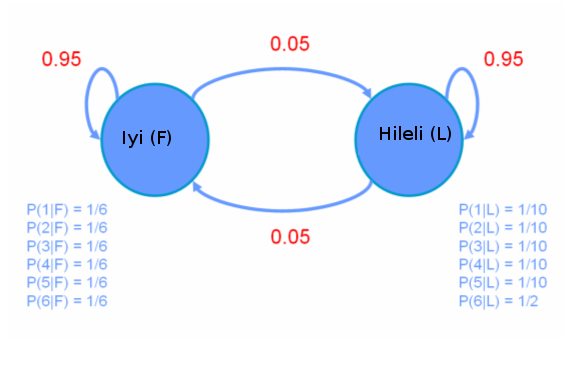
\includegraphics[height=6cm]{tser_hmm_09.png}

Üstteki modele göre hileli zardan 6 gelme olasılığı (salım olasılığı) daha
yüksek. İki saklı konum arasındaki geçiş anormal sayılmaz, ``arada sırada''
birinden bir konumdan diğerine geçiş var, kumarhane ``bazen'' zarları
değiştiriyor yani. Şimdi saklı geçişi bulalım,

\begin{minted}[fontsize=\footnotesize]{python}
import dhmm

rolls = [1,2,4,5,5,2,6,4,6,2,1,4,6,1,4,6,1,3,6,1,3,6,\
         6,6,1,6,6,4,6,6,1,6,3,6,6,1,6,3,6,6,1,6,3,6,1,\
         6,5,1,5,6,1,5,1,1,5,1,4,6,1,2,3,5,6,2,3,4,4]
rolls = np.array(rolls)-1
a = np.array([[0.95, 0.05],[0.05, 0.95]])
b = np.array([[1/6., 1/6., 1/6., 1/6., 1/6., 1/6.], 
              [1/10.,1/10.,1/10.,1/10.,1/10.,1/2.]])
pi = np.array([0.5, 0.5])

hmm = dhmm.HMM(2,6,pi,a,b)
print hmm.viterbi_path(rolls)
\end{minted}

\begin{verbatim}
[0 0 0 0 0 0 0 1 1 1 1 1 1 1 1 1 1 1 1 1 1 1 1 1 1 1 1 1 1 1 1 1 1 1 1 1 1
 1 1 1 1 1 1 1 1 1 1 0 0 0 0 0 0 0 0 0 0 0 0 0 0 0 0 0 0 0 0]
\end{verbatim}

Müthiş! Viterbi ile ne zaman hileli, ne zaman düzgün zar kullanıldığını pat
diye hesapladık. Kumarhane önce hilesiz başlıyor, ardından zarları
değiştiriyor ve uzun süre hile yapıyor. 

Algoritmanın nasıl işlediğini anlamak için farklı bir modele bakalım,

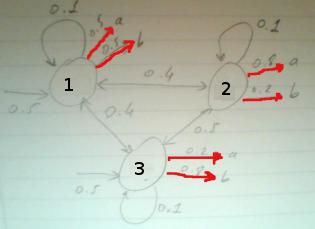
\includegraphics[height=6cm]{tser_hmm_03.png}

Bu modelde 3 tane saklı konum var, ve salım alfabesi $a,b$ (tabii kodlama /
matematiksel olarak 1,2 olacak). Viterbi algoritmasının işleyişini anlatmak
için saklı konumlar ve aralarındaki geçiş zamana doğru sağa doğru yayılacak
şekilde resimlenir, bu resme ``trellis'' deniyor.

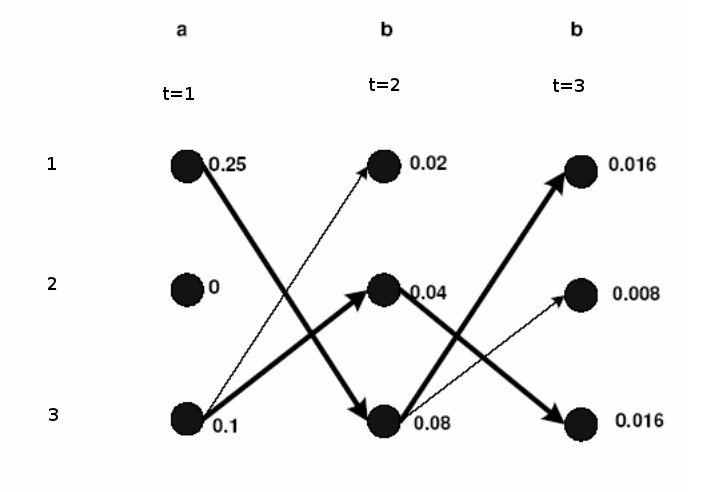
\includegraphics[height=6cm]{tser_hmm_08.png}

Kısayol algoritması şöyle; üstteki resimde zaman/konum düğümlerine
başlangıçtan o noktaya gelmenin olasılığı yazılmış. Yani bu değer o
noktanın ne kadar olası olduğunu gösteriyor. Hesabın bir örneği; trellisin
ortasından secelim, diyelim ki $t=1$ anında 3 konumundan 1 konumuna geçmek
istiyoruz, bu geçiş sonrası yol ne olur?  $t=1$'de 3 üzerinde 0.1 diyor,
3-1 geçişinin olasılığı 0.4 çarpı 1 konumundan 'b' salımı olasılığı 0.5, o
zaman 0.1*0.4*0.5 = 0.02. Böylece başla-3-1 yolunun olasılığı 0.02 haline
geldi. Bu hesap sağa doğru genişletilir, eğer bir noktaya birden fazla
geçiş mümkün ise, nihai hesaplar arasında en yüksek olan seçilir. En sağa
geldiğimizde 1'de biten bir 0.016 yolu görüyoruz, bir de 3'de biten bir
0.016 yolu görüyoruz. İki yolun hesabı aynı çıktı, çoğunlukla bu durum
olmaz, fakat bu yollardan herhangi birini seçmek, ya da ikisini birden
raporlamak problem değildir.

Yolu \verb!dhmm!'e hesaplatırsak,

\begin{minted}[fontsize=\footnotesize]{python}
import dhmm
a = np.array([[0.1,0.4,0.4],[0.4,0.1,0.5],[0.4,0.5,0.1]])
b = np.array([[0.5,0.5],[0.8,0.2],[0.2,0.8]])
pi = np.array([0.5, 0, 0.5])

hmm = dhmm.HMM(3,2,pi,a,b)
print hmm.viterbi_path([0,1,1])
\end{minted}

\begin{verbatim}
[0 2 0]
\end{verbatim}

Eğer 1 ve 3'e en soldan giriş yapan bir başlangıç noktası S, ve en sonda
tüm düğümlerin gittiği bir bitiş noktası E hayal edersek, aslında üstteki
tarif edilen [6] yazısında anlatılan kısayol algoritmasına
benziyor. Elimizde bir yönlü ve çevrimsiz bir çizit (directed, acyclic
graph) var, S'den başlıyoruz, sürekli adım atarak arkada bıraktığımız yolun
uzunluğunu (bu durumda olasılığını) sürekli toplayarak her adımda
hesaplıyoruz, ve hatırlıyoruz (gerçi üstteki örnekte olasılıklar çarpıldı
-çünkü o yolun birleşik olasılığı hesaplanmalıydı- fakat log alınıp
toplanabilirdi, hatta sayısal stabilite sebepleriyle bu
yapılmalıdır). Trellis'teki her geçiş çizitte bir kenar, daha önce
kullandığımız örnek $t=1$ anındaki 3-1 geçişi için kenar 0.4*0.5=0.2. Bu
kenarlar takip edilerek bir kısayol bulunacaktır.

Model Öğrenmek, İleri-Geri Algoritması

HMM'in güzellikleri bitmedi; sadece görünen semboller dizisini kullanarak,
sadece kaç tane saklı konum olacağını tanımlayarak, tüm HMM modelini
öğrenmek mümkün. Yani $A,B$ matrisleri, ve tabii ki bunu elde edince
görünen salımlara tekabül eden saklı geçişleri de
hesaplayabilecegiz. Kumarhane örneğine dönelim, yeni bir HMM yaratalım, ve
dışarıdan bir model tanımlamadan, onu direk veri ile eğitelim.

\begin{minted}[fontsize=\footnotesize]{python}
hmm2 = dhmm.HMM(2,6)
hmm2.train([rolls],iter=20)
print hmm2.viterbi_path(rolls)
print 'aic', hmm2.aic()
print hmm2.transmat
print hmm2.prior
print hmm2.obsmat
\end{minted}

\begin{verbatim}
[0 0 0 0 0 0 0 1 1 1 1 1 1 1 1 1 1 1 1 1 1 1 1 1 1 1 1 1 1 1 1 1 1 1 1 1 1
 1 1 1 1 1 1 1 1 1 1 0 0 0 0 0 0 0 0 0 0 0 0 0 0 0 0 0 0 0 0]
aic 233.31799296
[[ 0.97008754  0.02991246]
 [ 0.32816368  0.67183632]]
[ 0.5  0.5]
[[ 0.12184793  0.23208224  0.19549656  0.10143301  0.27422243  0.07491783]
 [ 0.18905143  0.2018225   0.17782606  0.17010257  0.01788689  0.24331055]]
\end{verbatim}

Saklı konum geçişleri aynı çıktı! Gerçi eğitimi birkaç kez işletmek gerekti,
çünkü HMM eğitimi bir tür Beklenti-Maksimizasyon (Expectation-Maximization -EM-)
algoritması kullanır, ve bu algoritmanın yerel maksimada takılıp kalması
mümkündür, o yüzden birkaç kez işlettik, ve AIC'si en düşük olanı seçtik. Fakat
bu zaten EM kullanıldığında uygulanması tavsiye edilen bir tekniktir.

Detaylara inmeden önce formülsel olarak, bize verili bir $V$ dizisi
bağlamında $t$ anında $i$ konumunda olmanın olasılığı lazım; yani 
$P(X_t = i | V; \lambda)$. Bu formüle nasıl erişiriz? $X_t = i$ ile $V$'nin
birleşik dağılımını düşünelim ($\lambda$'yi kalabalık olmasın diye
göstermiyoruz), onu $V$'leri ortadan bölerek iki parçalı olarak 
gösterebiliriz,

$$ P(X_t = i, V) = P( V_1,V_2,..,V_t,X_t=i) P (V_{t+1},V_{t+2},..,V_T | X_t=i )
$$

Eşitliğin sağ tarafındaki ilk kısım $\alpha$ ikinci kısım $\beta$ değil mi?
Evet. O zaman 

$$  = \alpha_t(i) \beta_t(i) $$

Fakat hala $V$'nin verili olduğu hali elde etmedik, onun için bir bölüm
lazım. Bölümü yapalım ve sonuca yeni bir sembol verelim,

$$ 
\gamma_t(i) \equiv P(X_t = i | V) = 
\frac{P(X_t = i, V) }{P(V)} = 
\frac{\beta_t(i)\alpha_t(i)}{ P(V)} 
$$

Bu noktada, teorik olarak, 

$$ \argmax_{1 \le i \le c} [ \gamma_t(i) ] $$

çözümü, yani $t$ anında $\gamma_t(i)$ maksimize edecek en iyi $X_t$
konumunu bulmak ve bunu tüm $t$'ler için yapmak bize verili $V$ için en
optimal saklı yolu verir diye düşünebilirdik, fakat üstteki ifade teker
teker konumlara bakıyor, ve geçişleri gözönüne almıyor. Bunun için Viterbi
algoritması hala en iyi çözüm. Detaylar için [1]. Her halükarda, üstteki
ifade bize eğitim için yardımcı olacak. 

Devam edelim, $\xi$'i tanımlayalım,

$$ \xi_t(i,j) = P(X_t = i, X_{t+1}= j | V; \lambda) 
\mlabel{2}
$$

$\xi$ ile $t$ anında $i$ konumunda $t+1$ anında $j$ konumunda olma
olasılığını tanımlamış oluyoruz. Üstteki ifadeyi 

$$  = \frac{\alpha_t(i)a_{ij}b_{j,V_{t+1}}\beta_{t+1}(j)  }{P(V;\lambda)}$$

olarak yazabiliriz, ve

$$  
= \frac{\alpha_t(i)a_{ij}b_{j,V_{t+1}}\beta_{t+1}(j)  }
{\sum _{i=1}^{c}\sum _{j=1}^{c} \alpha_t(i)a_{ij}b_{j,V_{t+1}}\beta_{t+1}(j)  }
$$

Bölendeki ifade bölünendeki ifadenin tüm $i,j$ üzerinden alınan toplamının
geriye sadece $P(V;\lambda)$ bırakacak olmasından ileri geliyor, çünkü (2)'den
hareketle bölünendeki ifade $P(X_t = i, X_{t+1}= j, V; \lambda) $. 

$\gamma_t(i)$'yi daha önce $V$'nin verildiği ve $\lambda$ modeli bilindiği
durumda $t$ anındaki saklı konum $i$'de olmak diye açıklamıştık. O zaman 
$\gamma_t(i)$ ve $\xi_t(i,j)$ arasında bir ilişki kurabiliriz,

$$ \gamma_t(i) =  \sum _{j=1}^{c} \xi_t(i,j) $$

Eğer $\gamma_t(i)$'nin tüm $t$'ler üzerinden toplamını alırsak, bu hesap
tüm zamanlar için $i$ konumunda olmanın, ya da $i$ konumundan başka
herhangi bir konuma geçmiş olmanın beklentisi olarak görülebilir (tabii en
son zaman indisi $T$'yi bu durumda toplamdan çıkartmak lazım, çünkü o
noktadan başka bir noktaya geçmek mümkün değil). Aynı şekilde
$\xi_t(i,j)$'nin $t=1,..,T-1$ üzerinden toplamını almak, bize konum $i$ ve
$j$ arasındaki tüm geçişlerin beklentisini verebilir.


$$ \sum _{t=1}^{T-1} \gamma_t(i) = \textrm{ i'den başka bir konuma geçiş beklentisi} $$

$$ \sum _{t=1}^{T-1} \xi_t(i,j) = \textrm{ i'den j'ye geçiş beklentisi} $$

Üstteki formülleri kullanarak HMM'in parametreleri $\lambda = (\pi,A,B)
$'yi tahminsel hesaplamak mümkündür. 

$$ \overline{\pi} = \textrm{t=1 anında i konumunda olma frekansı} = \gamma_1(i)
\mlabel{3}
$$

$$ \overline{a_{ij}} = \frac{\textrm{i konumundan j konumuna geçiş beklentisi}}
{\textrm{i konumundan başka herhangi bir konuma geçişin beklentisi}}
$$

$$  = \frac{ \sum _{t=1}^{T-1}\xi_t(i,j) }{ \sum _{t=1}^{T-1} \gamma_t(i) } 
\mlabel{4}
$$

$$ 
\overline{b_{j,k}} = 
\frac{\textrm{j konumunda olup } v_k \textrm{ sembolunu görmüş olmanın beklentisi}}
{j \textrm{ konumunda olmanın beklentisi} }
 $$

$$ = \frac{\sum _{t=1}^{T-1} \gamma_t(j) 1(V_t=k) }{\sum_{t=1}^{T-1}\gamma_t(j) } 
\mlabel{5}
$$

Tüm bunları kullanarak eğitim yaklaşımını şöyle belirleyebiliriz: bir
$\lambda=(\pi,A,B)$ modeli ile başla, ki başlangıç model rasgele değerler
ile bile tanımlanmış olabilir. Ardından formüller (3,4,5)'i kullanarak
$\overline{\pi},\overline{a_{ij}}$ ve $\overline{b_{j,k}}$'yi hesapla. Bu
hesap  ardından Baum ve arkadaşları  tarafından ispatlanmıştır ki [1]
$P(V;\overline{\lambda}) > P(V;\lambda)$, yani  yeni hesaplanan model
veriyi  eskisinden daha iyi açıklayacaktır.  O zaman  üstteki hesapları 
yeni hesaplanan $\overline{\lambda}$ ile tekrarlarsak, tekrar daha 
iyi bir model elde ederiz. Bunu ardı ardına yaparsak en optimal 
modele erişmiş oluruz. Bu yaklaşım aslında bir Beklenti-Maksimizasyon'dur (EM). 
Karışım modellerinde olduğu gibi akılda tutmak gerekir ki EM lokal
maksima'yı bulur, eğer bu maksimum nokta global (tüm modelin) maksimumu
değil ise yanlış bir noktada takılıp kalmış olabilir. Bu yüzden standart
tekniği burada da kullanıyoruz, farklı rasgele başlangıç noktalarından
başlatıp en iyi olurluğu rapor eden modeli nihai model olarak seçeriz. 

Sürekli Salımlar (Continuous Emissions)

Şimdiye kadar gördüğümüz ayrıksal HMM'ler her konumunda farklı bir ayrıksal
dağılıma göre zar atıyordu. A,B,C konumları olsun, A konumundan
ayrıksal dağılım $\left[\begin{array}{ccc} 0.2 & 0.5 &
    0.3 \end{array}\right]^T$'a göre zar atıyor olabiliriz, B konumunda
farklı bir ayrıksal dağılım $\left[\begin{array}{ccc} 0.4 & 0.5 &
    0.1 \end{array}\right]^T$'e göre zar atıyor olabiliriz.

Fakat HMM matematiği ayrıksal dağılımlar ile kısıtlı değildir. Her konumun
salım dağılımının ayrıksal olduğu gibi sürekli olması da mümkündür.

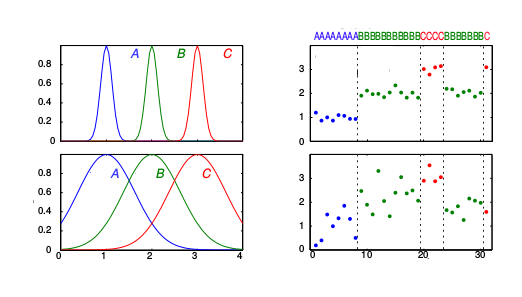
\includegraphics[height=6cm]{tser_hmm_10.png}

Üstteki resimde iki tane HMM gösteriyoruz, A,B,C diye tanımlı 3 konum var
(üst sıra bir HMM, alt sıra bir diğeri). Bu modele göre her konumda farklı
olan salım dağılımı ayrıksal değil, bir Gaussian. Mesela 1. HMM için A
konumunun mavi renkle gösterilen tek boyutlu bir Gaussian dağılımı var (sol
üst köşe), bu Gaussian $\mu=1$ üzerinden tanımlı, yeşil olan $\mu=2$,
vs. 1. HMM için örnek bir sürekli salım zinciri üst sağ köşedeki gibi
olabilir. Bir blokta 1 değeri etrafında bazı değerler görüyoruz, ardından 2
etrafında bir blok, sonra 3, sonra 2, böyle devam ediyor. Bu salım
değerlerine bakarak bir HMM'i eğitip hangi konumda hangi Gaussian olduğunu
ve konumlar arası geçiş olasılıklarını öğrenebiliriz! Resimde alt sırada
farklı Gaussian'lar ve (tabii ki) daha farklı salım zinciri var (saklı
geçiş zinciri aynı, ki bu durum modele uygun, fakat saklı zincir biraz daha
farklı da olabilirdi).

Sürekli dağılım bazlı HMM matematiği biraz daha farklı, bu konunun
detayları için [3, sf. 603]. Bu tür HMM hesapları için \verb!mhmm!
modülünü paylaştık. Bu modülle salım dağılımlarını hem çok boyutlu
Gaussian, hem de her konum için çok boyutlu {\em birkaç} Gaussian karışımı
olarak modelleyebiliriz. 

Bu modül ile [4, sf. 50]'de gösterilen deprem örneğini çözebiliriz.

\begin{minted}[fontsize=\footnotesize]{python}
import pandas as pd
df = pd.read_csv('earthquakes.txt',sep='\s*',header=None,index_col=0)
data = df[1]
data.plot()
plt.title('Depremler')
plt.savefig('tser_hmm_04.png')
\end{minted}

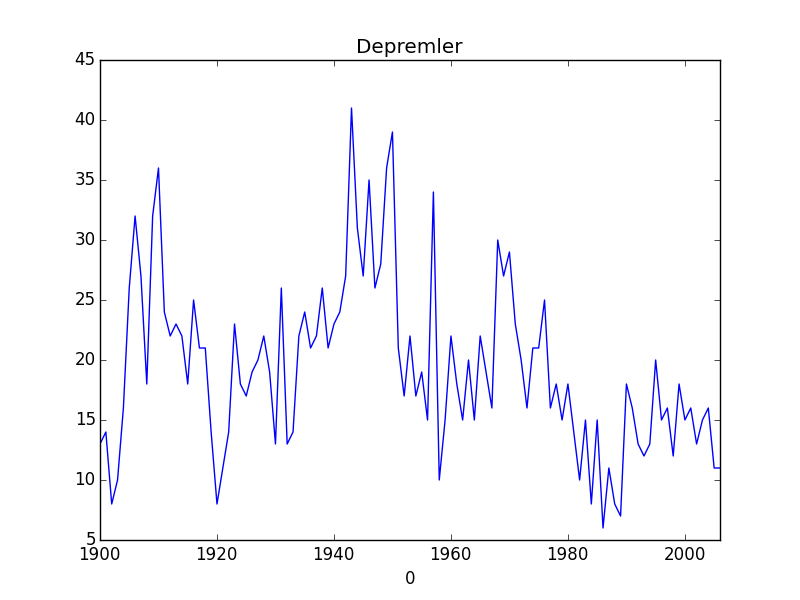
\includegraphics[height=6cm]{tser_hmm_04.png}

Üstteki grafikte dünyada her sene kaç tane büyük (Richter ölçeği 7 ve
üzeri) deprem olduğu gösteriliyor. Eşit büyüklükteki zaman aralıklarında
vuku bulan olayların sayısı çoğunlukla Poisson ile modellenir, ki [4]
problemi böyle çözmüş. Gaussian karışımları ile herhangi bir dağılımı
yaklaşıklayabileceğimizi biliyoruz, o zaman tek boyutlu iki Gaussian
karışımı üzerinden salımları modelleyebiliriz.  Kaç tane saklı konum
olmalı? [4]'te 2 ve 3 denenmiş; 2 konumlu durum depremlerin düşük seviyeli
ya da yüksek seviyeli zaman bloklarında meydana geldiği şeklinde
görülebilir. 3 konum veriyi düşük, orta, yüksek olarak ayırır. Bu
modellerden hangisi daha iyidir?

\begin{minted}[fontsize=\footnotesize]{python}
import mhmm
c=2
prior0 = np.ones(c) * 1/c
transmat0, _ = mhmm.mk_stochastic(np.random.rand(c,c))
d = np.reshape(data,(1,len(data),1))
hmm = mhmm.HMM(n_components=c, n_mix=2, startprob=prior0, 
               transmat=transmat0, covariance_type='diag')        
hmm.fit(dd)

print 'aic', hmm.aic()        
print hmm.score(d)
print hmm.transmat_
\end{minted}

\begin{verbatim}
(4, 1)
iteration 1, loglik = -344.981925
iteration 2, loglik = -339.666685
iteration 3, loglik = -338.222636
aic 696.445271513
[-337.77961902]
[[ 0.92211706  0.07788294]
 [ 0.06461021  0.93538979]]
\end{verbatim}

\begin{minted}[fontsize=\footnotesize]{python}
c=3
prior0 = np.ones(c) * 1/c
transmat0, _ = mhmm.mk_stochastic(np.random.rand(c,c))
d = np.reshape(data,(1,len(data),1))
hmm = mhmm.HMM(n_components=c, n_mix=2, startprob=prior0, 
               transmat=transmat0, covariance_type='diag')        
hmm.fit(d)
print 'aic', hmm.aic()        
print hmm.score(d)
print hmm.transmat_
\end{minted}

\begin{verbatim}
(6, 1)
iteration 1, loglik = -363.687193
iteration 2, loglik = -355.604032
iteration 3, loglik = -351.994401
iteration 4, loglik = -347.108994
iteration 5, loglik = -341.249047
iteration 6, loglik = -336.556782
iteration 7, loglik = -333.417138
aic 702.834275264
[-331.17921244]
[[ 0.85777432  0.10857336  0.03365233]
 [ 0.16314564  0.70421656  0.1326378 ]
 [ 0.05122129  0.16358917  0.78518954]]
\end{verbatim}

Her iki örnek için geçiş matrisi [4, sf. 51]'de gösterilen sonuçlara
oldukça yakın çıktı. AIC sonuçlarına göre 2 saklı konumlu model 3 saklı
modelliden biraz daha iyi gibi duruyor. AIC değerleri de [4. sf. 91]'de
raporlanan değerlere oldukça yakın.

Ses Tanımak

Bir ses kaydı zaman dilimlerinin birbiri ile bağlantılı olduğu bir zaman
serisine örnektir. \verb!rec.py! ile istediğimiz sesi bilgisayarımızın
mikrofonu ile kaydedebiliriz. Bizim önceden kaydettiğimiz bazı sesler altta,

\begin{minted}[fontsize=\footnotesize]{python}
import scipy.io.wavfile
from scikits.talkbox.features import mfcc

sample_rate, computer = scipy.io.wavfile.read('computer.wav')
sample_rate, emacs = scipy.io.wavfile.read('emacs.wav')
sample_rate, nothing = scipy.io.wavfile.read('nothing.wav')
\end{minted}

\begin{minted}[fontsize=\footnotesize]{python}
plt.plot(computer)
plt.title('Computer')
plt.savefig('tser_hmm_05.png')
plt.hold(False)
plt.plot(emacs)
plt.title('Emacs')
plt.savefig('tser_hmm_06.png')
plt.hold(False)
plt.plot(nothing)
plt.title('Nothing')
plt.savefig('tser_hmm_07.png')
plt.hold(False)
\end{minted}

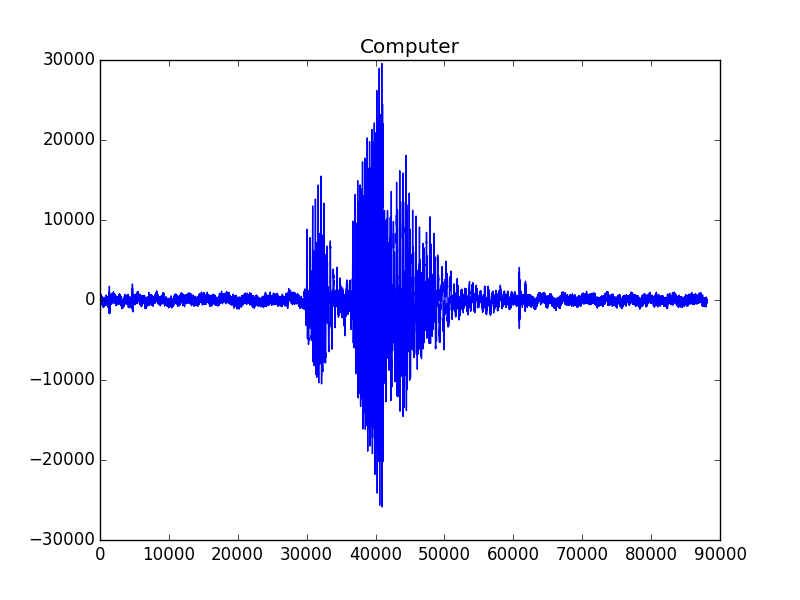
\includegraphics[height=6cm]{tser_hmm_05.png}
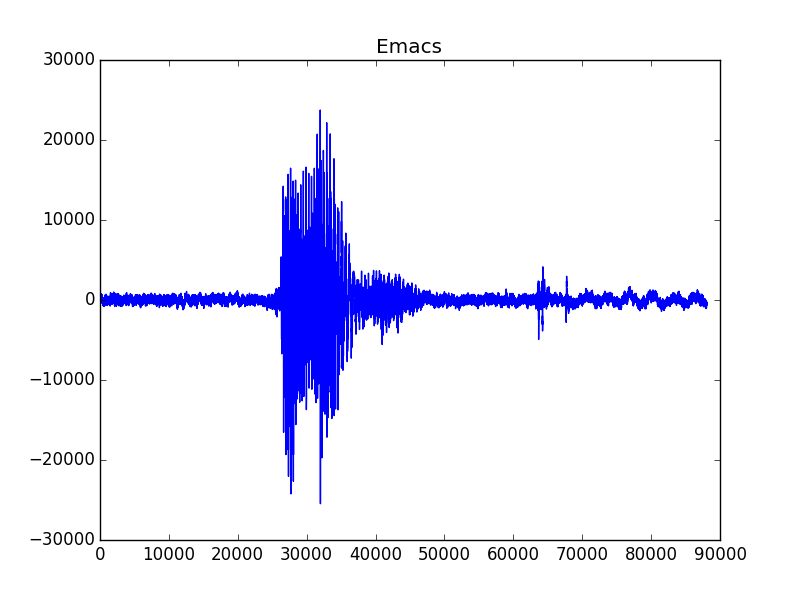
\includegraphics[height=6cm]{tser_hmm_06.png}
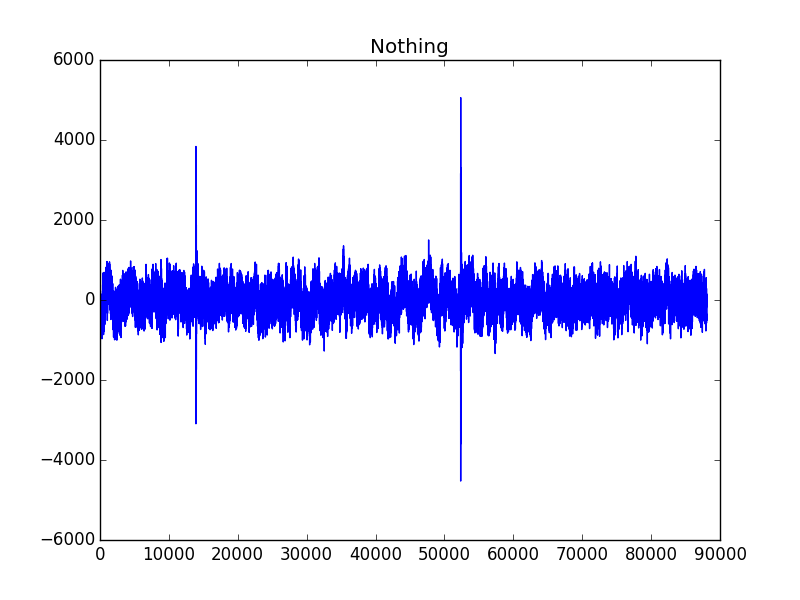
\includegraphics[height=6cm]{tser_hmm_07.png}

HMM'ler ses tanıma için biçilmiş kaftan. Fakat genellikle üstteki zaman
serileri direk oldukları şekilde kullanılmazlar. Ses kayıtları belli
dilimlere bölünerek, o bölümler üzerinde özellik çıkarımı (feature
extraction) uygulanır. Bu özelliklerden en popüleri Mel Frekansı Cepstral
Katsayıları (MFCC). Alttaki çağrıyla 2 saniyelik kaydımız üzerinde MFCC
hesabını görüyoruz,

\begin{minted}[fontsize=\footnotesize]{python}
from scikits.talkbox.features import mfcc
ceps_c, mspec, spec = mfcc(emacs)
print 'ses kaydi', len(emacs) , 'boyut', ceps_c.shape
print len(emacs) / 549
\end{minted}

\begin{verbatim}
ses kaydi 88064 boyut (549, 13)
160
\end{verbatim}

Eğer HMM'ses tanımak için kullanmak istiyorsak HMM eğitimini üstte
boyutları gösterilen MFCC vektör dizisi üzerinde uygularız. HMM salımı 13
boyutlu bir Gaussian karışımı olur (karışım sayısı uygulamaya göre farklı
olabilir). Optimal saklı konum sayısı AIC üzerinden saptanır. Her bilinen
ses kaydı için ayrı bir HMM eğitilir, mesela 'emacs' kaydı için bir HMM,
'computer' sesi için ayrı bir HMM... Nihai uygulama ise mikrofondan gelen
sesleri 2. saniyelik kısımlara bölerek üzerlerinde yine aynı MFCC hesabını
yapar, ve bu vektör dizisinin ne kadar olası olduğunu her HMM'e
``sorar''. Hangi HMM daha iyi olurluk rapor ediyorsa ses o etikete aittir.

Ödev: Ekteki \verb!mic.py!'da mikrofondan sürekli gelen verilerin işlenmesi
gösteriliyor, bu örnek üstteki teknik ile HMM için uzatılabilir.


Kaynaklar 

[1] Rabiner, {\em A Tutorial on Hidden Markov Models and Selected Applications in Speech
Recoognition}

[2] Shalizi, {\em Statistics, Chaos, Complexity and Inference Lecture}

[3] Murphy, {\em Machine Learning, A Probabilistic Perspective}

[4] Zuccini, {\em Hidden Markov Models for Time Series}

[5] Bayramli, Lineer Cebir, {\em Ders 21}

[6] Bayramli, Bilgisayar Bilim, {\em Dinamik Programlama}

\end{document}
